\documentclass[12pt]{article}
\usepackage[pdftex]{graphicx}
\usepackage{multicol}
\title{GEOMETRY!!!!! Computational Geometric Analysis on Surfaces}
\pagestyle{plain}
\author{Alex Henniges \\ Thomas Williams \\ Mitch Wilson \\ \\ University of Arizona Undergraduate Research Program\\
Supervisor: Dr. David Glickenstein\\
}
\date{July 7, 2008}
\begin{document}
	\maketitle
	%\begin{center} By: Alex Henniges, Thomas Williams, Mitch Wilson 
  %\end{center}
  %Supervisor: Dr. David Glickenstein, University of Arizona, Summer 2008
  %\LaTeX{} is a document preparation system for the \TeX{} 
  %typesetting program. It offers programmable desktop publishing 
  %features and extensive facilities for automating most aspects of 
  %typesetting and desktop publishing, including numbering and 
  %cross-referencing, tables and figures, page layout, bibliographies, 
  %and much more. \LaTeX{} was originally written in 1984 by Leslie 
  %Lamport and has become the dominant method for using \TeX; few 
  %people write in plain \TeX{} anymore. The current version is 
  %\LaTeXe.
  % This is a comment, it is not shown in the final output.
  % The following shows a little of the typesetting power of LaTeX
  %\begin{eqnarray}
    %E &=& mc^2                              \\
    %m &=& \frac{m_0}{\sqrt{1-\frac{v^2}{c^2}}}
    %X &=& V - E + F\\
    %K_i &=& 2\pi - \sum{\angle i \forall \nabla}
  %\end{eqnarray}
  %For surfaces that are representations of a sphere, $X = 2$. In the case of a regular torus, $X = 0$. 
  \newpage
  \section{Introduction}
  \maketitle
  Over the course of this summer, we examined and learned about various topological and geometric manipulations across various dimensional objects. We use a lot of C++ to code our work, and have a lot of work to show for it. In section we will introduce the concepts behind our project, as well as discuss our plan of action. 
  Things we ought to put here:
  \begin{itemize}
  \item Definitions, like triangulations and such
  \item A basic verbal-type background of what we are doing, not too many equations
  \item Our aspect of what we are doing
  \item Our interpretation of the end goal
  \item What we aim to accomplish over the course of the summer
  \end{itemize}
  
  \subsection{Introduction to triangulations and circle packing}
  \maketitle
  Suppose you are asked to make a sphere, but are only given a small number of edges, vertices, or faces to work with. What do you do? In geometry, a common question asked is how to make representations of complex shapes with as little stuff as possible. In fact, you are probably already familiar with the most basic representation of a sphere- a tetrahedron. Using only four vertices, six edges, and four faces, the tetrahedron is able to give us an approximation to a sphere. Similarly, three vertices (a triangle) can be used to approximate a circle in two dimesnions. Naturally, if we add more vertices, we are able to better illustrate our shapes. \newline
  
   \noindent Of course, spheres aren't the only things geometers care about. Another shape of large interest is known as the torus. It looks like a donut. It turns out that you can make a visualization of this object using only 7 vertices \cite{lutzmanifold}. With more vertices the shape becomes better curved and reminiscent of breakfast. Mmm, torus. It is also possible to add $''handles''$ to any shape, resulting in the addition of another torus. There are also various other shapes which can be represented with varying numbers of vertices, like Klein bottles and cross-caps.\cite{WolfMath} has more information on these fascinating shapes.\newline
   
   \noindent Like in modern video games and Hollywood movies, we can generate various shapes of many different sizes using polygons that mold to form the special effect. For these and all shapes, we will focus on building them solely out of triangles. Since any regular polygon can be broken up into smaller triangles, we can essentially represent any shape with enough vertices. We define a shape as $triangulizable$ if we can connect all triangles in a particular fashion such that they create a closed 3-dimenional shape.\newline
  
\begin{figure}
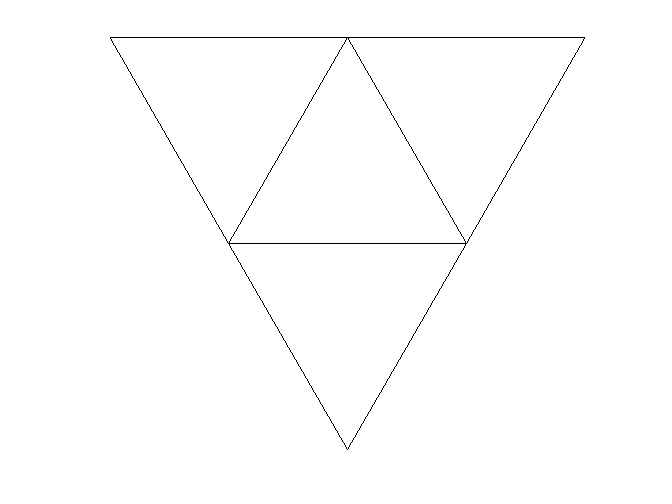
\includegraphics[scale = 0.5]{flattetrahedron.png}
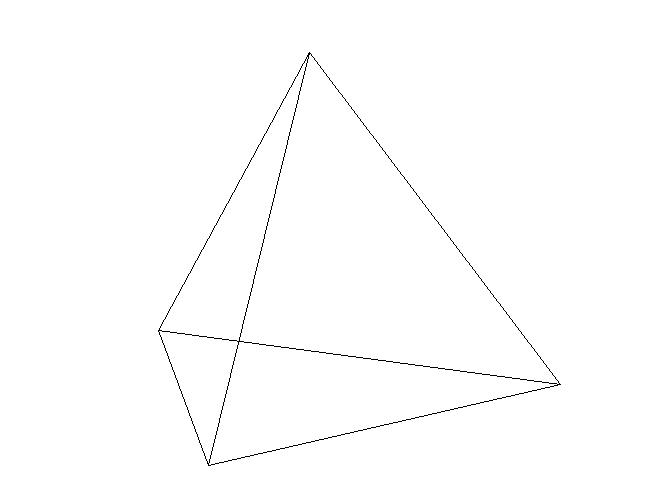
\includegraphics[scale = 0.3]{tetrahedron.jpg}
\caption{An example of triangulation. A triangle can be folded up into a tetrahedron.}
\end{figure}

\noindent An issue arises regarding the uniqueness of these triangulations. There are over 28 $trillion$ ways to triangulate a sphere using only 23 vertices. It is currently unknown how many ways a single torus can be made using that number of vertices (to us, at least). However, all toruses do share something very peculiar, as do all sphere configurations. The Euler characteristic, $\chi$, is a value associated with three dimensional shapes. It is defined as $\displaystyle\chi = V - E + F$, where $V, E, $and $F$ are the number of vertices, edges, and faces a given manifold has. Certain shapes have the same $\chi$ value. For example, any torus has $\chi = 0$, and any representation of a sphere has $\chi = 2.$ Table \ref{EuChar} has listings for many common shapes. 

\noindent While we can indicate how these different vertices are connected to each other, there is still an issue regarding the lengths of these edges. There are an infinite number of possible edge length configurations just as there are an infinite number of possible triangles. We introduce a method known as circle packing to quantify edge lengths. In circle packing, the shapes in question can be constructed using circles of the same dimension on each of the vertices. Circles can be used to make the sides of a polygon; spheres can be used to make the edges of a polyhedron. These shapes are mutually tangent to each other, and two radii make up one edge. Thus, the length is simply the sum of the two radii of the adjacent vertices.
  
  \begin{eqnarray*}
  l_{ij} = r_i + r_j
  \end{eqnarray*}
  
\begin{figure}
\begin{center}
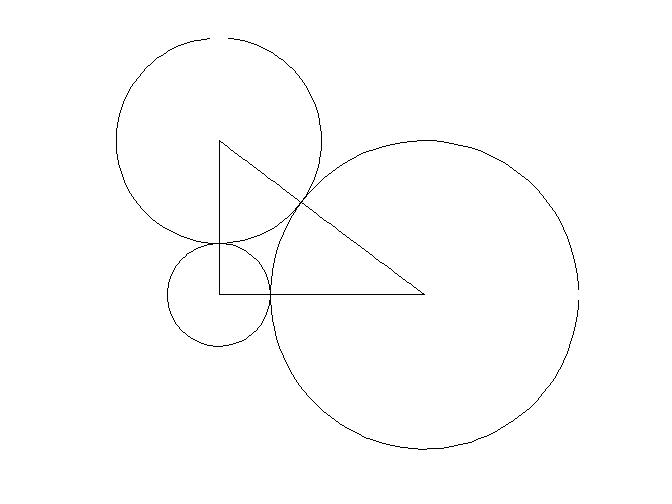
\includegraphics[scale = 0.3]{righttriangulation.jpg}
\end{center}
\caption{An example of circle packing. Three mutually tangent circes forming the perimeter of a triangle.}
\end{figure}

\begin{table}
\begin{tabular}{ccccc}
\label{EuChar}
Name  &	Vertices, V &	Edges, E & Faces, F &	$\chi, V - E + F$\\
\hline 
Tetrahedron &	4 &	6 &	4 &	2\\
Hexahedron or cube &	8 &	12 &	6 &	2\\
Octahedron 	&	6 &	12 &	8 & 2\\
Dodecahedron 	&	20 &	30 &	12 &	2\\
Icosahedron &	12 & 30 & 20 &	2\\
Torus & 9 & 27 & 18 & 0\\
Double torus & 10 & 36 & 24 & -2
\end{tabular}
\caption{Listings of vertices, edges, and faces for some common shapes \cite{wiki}}
\end{table}

\begin{figure}
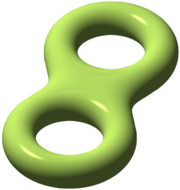
\includegraphics{180px-Double_torus_illustration.png}
\caption{This is a double torus. It has $\chi$ = -2.}
\end{figure}

 % At the beginning of this project, some of us only had a vague idea about what our end goal was. Each of us had varying levels of familiarity with geometry. Some of us have taken college courses in it, some of us haven't touched geometry since freshman year of high school. However, it quickly became clear that we were all really into this topic and used what skills we did have to tackle the situation. 
%  
%  Our problem involves the adaptability of surfaces over time to reach an end shape. While our initial focus was on simple, closed surfaces that we would be able to visualize undegoing its transformation without the use of software, we also began investigating more complex triangulations in hopes of better grasping the whole subject. 
  \subsection{Combinatorial Ricci flow}
  \maketitle  
Just because we have a triangulation and that it is circle packed does not mean that it is already compact and organized. Vertices can be too large or too small, and the end shape can be somewhat repulsive. We would like to have a way to make these radii as uniform as possible while keeping the original shape intact. We introduce the equation for combinatorial Ricci flow, which allows an individual radius to change over time. The differential equation can be written as 
  \begin{equation}
  \frac{dr_i}{{dt}} = -K_ir_i
  \end{equation}
  
\noindent where $K_i$ is a characteristic called the curvature of a vertex, and $r_i$ is the radius or weight of the vertex in terms of dimensions. The value of $K_i$ changes with time. Its value is found by determining the angles of all triangles containing vertex $i$. Using side lengths (or radii) we can determine the angle using the law of cosines. For a triangle with lengths $a, b$ and $c,$ the angle opposite side $c$ is:
  
  \begin{eqnarray*}
  \angle C = \arccos\frac{a^2 + b^2 - c^2}{2ab}
  \end{eqnarray*} 
  
\noindent with similar formulas for the other angles. We take the sum of all angles associated with a vertex $i$ and define the curvature $K_i$ as:

  \begin{equation}
  K_i = 2\pi - \sum{\angle i}
  \end{equation}
  
\noindent So since the differential equation depends on a variable whose value changes over time, we cannot solve it so easily.\newline
   
\noindent An issue we noted that would happen is that based on the equation, more often than not, the lengths of the radii would decrease. Take the example of a simple tetrahedron with all sides of equal length, we find that the curvature of each vertex always equals $\pi$. Thus in solving the differential equation computationally we would decrease each vertex by the same amount, but the curvature of each vertex would still remain $\pi$. The radii would continue to decrease until they approach zero length. We then have to address that issue since computers don't like working with numbers near zero, as in the denominator of the arccosine function. Weird, unwanted stuff might happen. Let us introduce the ability to resize the length of each radius by a scalar, $\alpha$. We denote each scaled length by $\tilde{r_i}$ and equate as
 
 \begin{equation}
 \tilde{r_i} = \alpha r_i
 \end{equation} 
 
\noindent Thus in plugging in to the differential equation we get
 
 \begin{eqnarray}
 \label{ref1}
 \frac{d\tilde{r_i}}{dt} &=& \frac{d(\alpha r_i)}{dt} = \alpha \frac{dr_i}{dt} + r_i\frac{d\alpha}{dt}\nonumber\\
 &=& -\alpha K_ir_i + \frac{\tilde{r_i}}{\alpha}\frac{d\alpha}{dt} \nonumber \\
 &=& -\tilde{K_i}\tilde{r_i} + \frac{\tilde{r_i}}{\alpha}\frac{d\alpha}{dt}
 \end{eqnarray}
 
\noindent Since we are scaling all sides by the same factor, this does not effect the curvature of the surface, so $\tilde{K_i} = K_i$. It also turns out that $$\displaystyle \frac{1}{\alpha} \frac{d\alpha}{dt} = \frac{d(\mbox{log}~\alpha)}{dt}$$ 
 In order to find an appropriate value for $\alpha$ we decided to use the following criteria:
 
\begin{equation}
\label{eqprod}
\prod{\tilde{r_i}(t)} = \prod{\tilde{r_i}(0)} = \prod{\alpha r_i(0)} = C\mbox{, a constant}
\end{equation}

\noindent This can be used to prevent radii from decreasing to zero. It turns out if you take the derivative of ($\ref{eqprod}$) with respect to time you find that 
 
\begin{equation}
\frac{d(\mbox{log}~\alpha)}{dt} = \frac{\mbox{sum of all curvatures}}{\mbox{number of vertices}} = \overline{K}, \mbox{average curvature}
\end{equation}
 
\noindent It turns out that $\overline{K}$ is constant for any iteration of our triangulation and is equal to $\displaystyle\frac{2\pi\chi}{|V|}$, where $|V|$ is the number of vertices and $\chi$ is the Euler characteristic. Plugging this back into ($\ref{ref1}$) we determine that

\begin{equation}
\frac{d\tilde{r_i}}{dt} = -\tilde{K_i}\tilde{r_i} + \overline{K}\tilde{r_i} = (\overline{K} - K_i)\tilde{r_i}
\end{equation}

\noindent However, since everything is now a function of $\tilde{r_i}$ and not $\alpha$, we can treat $\alpha$ as a constant and thus $\displaystyle\frac{d\alpha}{dt} = 0$. Therefore, we can easily plug $\tilde{r_i} = \alpha r_i$ back in to the differential equation, so we end up with:

\begin{eqnarray}
\frac{d\tilde{r_i}}{dt} &=& (\overline{K} - K_i)\tilde{r_i} \nonumber \\
\alpha\frac{dr_i}{dt} &=& (\overline{K} - K_i)\alpha r_i \nonumber \\
\frac{dr_i}{dt} &=& (\overline{K} - K_i)r_i
\end{eqnarray}

\noindent This is known as normalized Ricci flow, as in \cite{chowluo}. In the case of the basic tetrahedron, the radii would not change after each iteration as $\overline{K} = K_i = \pi$ for each vertex and thus $\displaystyle\frac{dr_i}{dt} = 0$. 

\newpage
\section{Analysis/Results}
\maketitle
  This might be where we can discuss what we've accomplished, maybe put in a couple pictures, or at least hypothetical illustrations. That'd be cool.\newline
  
  Here we will discuss some of the things that we have been working on, as well as document examples to show correctness.
  
  \subsection{Geometric layout}
  \maketitle
  
  We decided to use a set of arrays that would allow us to sort all the required data, mapping each element in one set to another in another array. While this may seem redundant, we felt that it made it easier to access data, as well as make sure that everything was conncted properly.\newline
  
  We structured our data into the following format\newline
  
  \begin{center}
  \begin{tabular}{|c|c|c|}
  \hline
  Vertices & Edges & Faces\\
  \hline
  adjacent vertices & component vertices & component vertices\\
  constructed edges & adjacent edges & component edges\\
  constructed faces & construced faces & adjacent faces\\
  \hline
  \end{tabular}
  \end{center}
  
\begin{figure}
\includegraphics[scale = 0.5]{triangulationUML.png}
\caption{a list of some commands we have written so far}
\end{figure}

\subsection{Solving the Ricci flow ODE}
\maketitle
After investigating various methods to run our differential equation, we opted to use a Runge-Kutta format, which has numerous benefits over the simpler but less efficient Euler method. According to $\cite{DiffEq}$ the error associated with using Runge-Kutta is on the order of $h^4$, whereas with a standard Euler approximation the error is simply of order $h$, with $h$ being our step incremental. For initial runs, we are using a value of $h = 0.001$.\newline
  
  \begin{figure}
  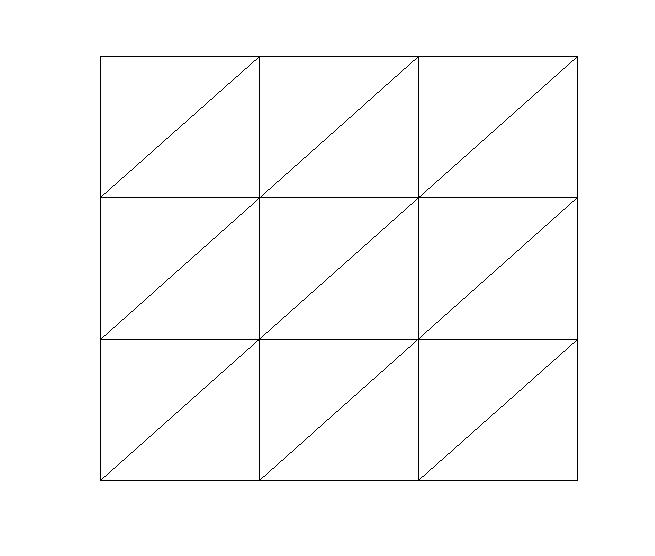
\includegraphics[scale = 0.4]{torus2.jpg}
  \caption{A triangulation of the torus. Like-numbered vertices are connected together.}
  \end{figure}

\subsection{Converting known triangulations}
\maketitle

\noindent While we are able to manually construct a few basic triangulations by hand, as we add more vertices that will become ever harder. \cite{lutzmanifold} has millions of known triangulations of varying size. However, the format is different than our setup, so we developed an algorithm to take a given triangulation, saved on its own as a text file, and be able to convert it into the form that we use. We were able to transform this
  
 \begin{verbatim}{manifold_lex_d2_n5_o1_g0_#1=[[1,2,3],[1,2,4],[1,3,4],
 [2,3,5],[2,4,5], [3,4,5]]}
 \end{verbatim}
 
into this:
\begin{multicols}{3}{
\begin{verbatim}
Vertex: 1
2 3 4
1 2 4 
1 2 3 
Vertex: 2
1 3 4 5
1 3 5 7 
1 2 4 5 
Vertex: 3
1 2 4 5
2 3 6 8 
1 3 4 6 
Vertex: 4
1 2 3 5
4 5 6 9 
2 3 5 6 
Vertex: 5
2 3 4
7 8 9 
4 5 6
Edge: 1
1 2
2 3 4 5 7 
1 2 
Edge: 2
1 3
1 3 4 6 8 
1 3 
Edge: 3
2 3
1 2 5 6 7 8 
1 4 
Edge: 4
1 4
1 2 5 6 9 
2 3 
Edge: 5
2 4
1 3 4 6 7 9 
2 5 
Edge: 6
3 4
2 3 4 5 8 9 
3 6 
Edge: 7
2 5
1 3 5 8 9 
4 5 
Edge: 8
3 5
2 3 6 7 9 
4 6 
Edge: 9
4 5
4 5 6 7 8 
5 6 
Face: 1
1 2 3 
1 2 3 
2 3 4 
Face: 2
1 2 4 
1 4 5 
1 3 5 
Face: 3
1 3 4 
2 4 6 
1 2 6 
Face: 4
2 3 5 
3 7 8 
1 5 6 
Face: 5
2 4 5 
5 7 9 
2 4 6 
Face: 6
3 4 5 
6 8 9 
3 4 5
\end{verbatim}
}\end{multicols}

\subsection{Flips}
\maketitle

\subsection{Adding/removing vertices}
\maketitle

\subsection{Adding toruses}
\maketitle

\subsection{Special cases}
\maketitle
  
  \newpage
  \section{Future Work}
  
  \maketitle
  \cite{DrG}
  \cite{chowluo}
  
  Dual lengths, dual areas. The stuff inside the triangles, etc. 
  
  Not just circle packing, let the circles overlap and introduce a second weight $\phi$. We can then evaluate our side lengths as $$l_{ij} = \sqrt{r_i^2 + r_j^2 + 2r_ir_j\cos(\Phi(e_{ij}))}$$ With this more general interpretation, we can examine questions asked by Chow and Luo in \cite{chowluo}.  
  
  We would also like to start investigating 3-dimensional constructs. We can adjust our current code as much as we need to, and ultimately be able to evaluate Yamabe flow, as discussed by \cite{DrG}. We can also try and investigate how our code applies (if it does) to hyperbolic and spherical coordinates.  
  
  \newpage
  \section{Conclusions}
  
  We learned a lot of things along the way.\newline
  
  \noindent We would like to thank Dr. David Glickenstein for having us on this project, Dr. Robert Indik and the University of Arizona Math Department for their help and support, and the VIGRE foundation for making this all possible. 
  \maketitle
   
  \newpage
  \bibliography{Test1}  
  \bibliographystyle{plain}
  
  \newpage
  \subsection*{About the Authors}
  \maketitle
  
  Alex Henniges is a junior double majoring in Math and Computer Science. Plus he's cool. \newline
  
  \noindent Thomas Williams is a senior in Comprehensive Mathematics with a minor in Computer Science and a strong background in Math Education. He's cool, too. \newline
  
  \noindent Mitch Wilson is a senior majoring in Applied Math and Mechanical Engineering. He's ok. 
\end{document}